\documentclass[conference]{IEEEtran}
\IEEEoverridecommandlockouts
% The preceding line is only needed to identify funding in the first footnote. If that is unneeded, please comment it out.
\usepackage{cite}
\usepackage{amsmath,amssymb,amsfonts}
\usepackage{graphicx}
\usepackage{textcomp}
\usepackage{xcolor}
\usepackage{algorithm} 
\usepackage{algpseudocode} 
\def\BibTeX{{\rm B\kern-.05em{\sc i\kern-.025em b}\kern-.08em
    T\kern-.1667em\lower.7ex\hbox{E}\kern-.125emX}}
\begin{document}

\title{Simulated Annealing Approach to ICCAD Contest Problem A: Reinforcement Logic Optimization for a General Cost Function\\}


\author{\IEEEauthorblockN{1\textsuperscript{st} Oniontow Ren-Xuan Wang}
\IEEEauthorblockA{\textit{Department of Electrical Engineering} \\
\textit{of National Taiwan University}\\
Taipei, Taiwan. \\
}
\and
\IEEEauthorblockN{2\textsuperscript{nd} Boyuan Cheng}
\IEEEauthorblockA{\textit{Department of Electrical Engineering} \\
\textit{of National Taiwan University}\\
Taipei, Taiwan. \\
}
\and
\IEEEauthorblockN{3\textsuperscript{rd} Stanley Huang}
\IEEEauthorblockA{\textit{Department of Electrical Engineering} \\
\textit{of National Taiwan University}\\
Taipei, Taiwan. \\
}
}

\maketitle

\begin{abstract}
This is the final report of Introduction to Electronic Design Automation, using simulated annealing technique to resolve problem A of ICCAD contest 2024.
The overall process comprises two main phases: logic synthesis and technology mapping. Logic synthesis was conducted using the Berkeley ABC tool, applied specifically to design1-6.v within the ICCAD contest benchmark. Our evaluation revealed that certain cost estimators show significant performance improvements during the logic synthesis phase, whereas technology mapping exhibited minimal impact. Conversely, other cost estimators indicated that the logic synthesis phase had negligible effects, while technology mapping performed admirably.
\end{abstract}

\begin{IEEEkeywords}
simulated annealing, logic synthesis, handsome but somewhat stupid oniontow
\end{IEEEkeywords}

\section{Problem Description}

We have been provided with a specified netlist in Verilog format, a cell library in a JSON-like format containing parameters for various primitive gates, and a black-box cost estimator.

\subsection{Netlist}

The input netlist is a flattened netlist in Verilog format without hierarchy (one top module only).\\
The netlist is composed of:
\begin{itemize}
    \item primitive gates (and, or, nand, nor, not, buf, xor, xnor)
    \item wires
    \item constant values (1’b1, 1’b0)
\end{itemize}
All primitive gates are assumed to have only 2 inputs and 1 output
except for buffer and not gates, which have only 1 input and 1 output.
All primary inputs and primary outputs are scalars (i.e., one-bit signals)\\

\subsection{Cell library}

For each primitive gate, there exists at least one corresponding cell in the cell library. The document comprises two main sections, each structured as a JSON object. The first section includes three properties: cell\_num, attribute\_num, and attributes.
\begin{itemize}
\item cell\_num: Indicates the total number of cells available in the library.
\item attribute\_num: Specifies the number of attributes associated with each cell.
\item attributes: A JSON array listing the attribute names for each cell.
\end{itemize}
The second section, labeled cells, is also represented as a JSON array. This section contains exactly cell\_num entries, each detailing exactly attribute\_num properties. An illustrative excerpt from the cell library is provided in Figure 1.

The second section is cells, which is a JSON array. There are exactly \#cell\_num cells described in this section. For each cell, exactly \#attribute\_num properties are specified. Fig. 1 shows an example of part of the cell library.
\begin{figure}
    \centering
    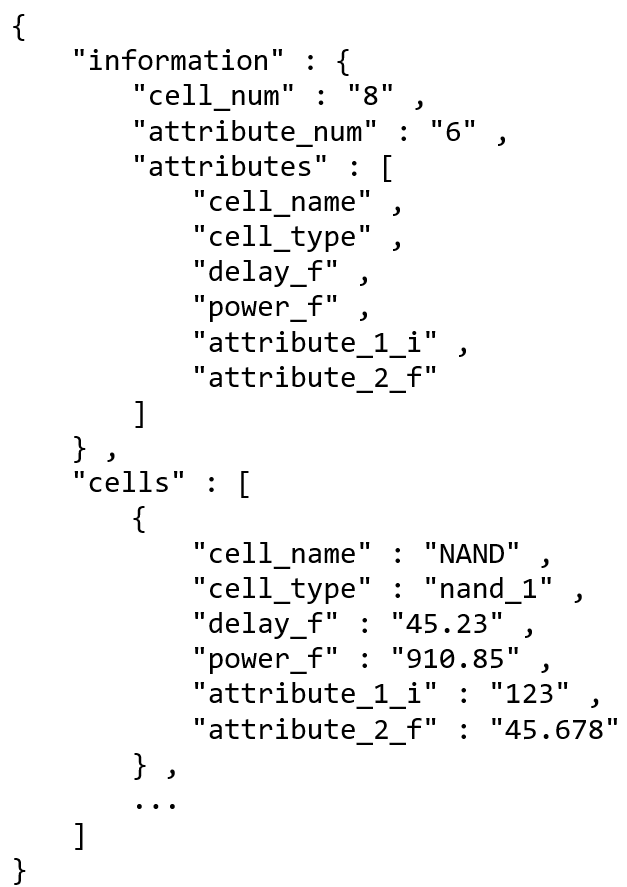
\includegraphics[width=0.6\linewidth]{example of cell library.png}
    \caption{Example of cell library}
    \label{fig:enter-label}
\end{figure}

\subsection{Cost Function Estimator}

The cost function estimator is an executable file that accepts two input files and produces one output file. The input files consist of a cell library and a netlist, where all gates in the netlist are defined by the cell library. The resulting output file provides a floating-point number representing the cost associated with the netlist.

\section{Simulated Annealing Strategy}

Upon receiving a netlist, our primary objective is to perform logic synthesis and reduction, predicated on the assumption that a reduced number of gates correlates with lower costs in terms of area, power, or other relevant properties. Following the logic synthesis, we obtain a gate-level Verilog file, which is subsequently mapped to the gates specified in the cell library.

To enhance performance further, we identify gates within the cell library that are more compatible with the given cost estimator. These gates are utilized for swift technology mapping of the logic gates during the logic reduction phase and serve as the initial condition for the subsequent technology mapping phase. We employ the simulated annealing method to achieve an acceptable cost. Figure 2 illustrates the flowchart of our process.

\begin{figure}
    \centering
    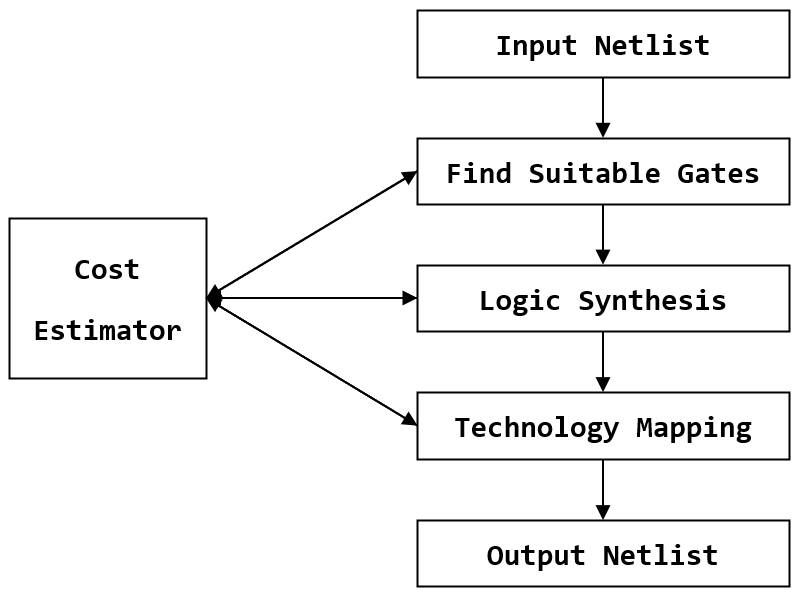
\includegraphics[width=1\linewidth]{flow chart.png}
    \caption{Flow Chart of Overall Process}
    \label{fig:enter-label}
\end{figure}

\subsection{Find Suitable gates}

For the initial part, we create a fake netlist that contains only one of each primitive gate. Then, we assign each gate all possible types and greedily pick the best assignment for the netlist. By performing this process for all primitive gates, we obtain a dictionary that contains the best types for each primitive gate. Below is the pseudo code for finding the most suitable gates:

\begin{algorithm}
\begin{algorithmic}[1]
    \caption{Find-Suitable-Gates}\label{euclid}
    \State BestType = $\emptyset $
    \For {gate $\in$ gates}
    \State CurrentBest $\gets \infty$ 
        \For {type $\in $ types}
            \If {CostEstimator(gate[type]) $<$ CurrentBest}
                \State CurrentBest $\gets$ type
            \EndIf
        \EndFor
        \State BestType $\gets $ BestType $\cup $ \{gate:CurrentBest\}
    \EndFor
    \State \Return BestType
\end{algorithmic}
\end{algorithm}

\subsection{Logic Synthesis}

For the logic synthesis part, we conduct operations on the netlist with the help of Berkeley ABC. We first convert the netlist to an And-Inverter-Graph (AIG) and then perform simulated annealing on the AIG. The simulated annealing process is defined with the following conditions:

\subsubsection{Action Space}

Action space of the logic synthesis process is a set of some ABC commands such as $resyn$, $fx$, $compress$, $dc2$ $\dots$ .

\subsubsection{Neighborhood Structure}

The neighborhood of each AIG is all AIGs produces by conducting one command in the action space.

\subsubsection{Cost Function}

Cost function is defined by the given cost estimator.\\

In every iteration of the simulated annealing loop, we randomly jump to a neighboring state. We then map the current AIG to a netlist output in Verilog format using the dictionary of the most suitable gates, if available. If not, we assign all gates to type I for time-saving considerations. After mapping, we obtain the cost from the cost estimator. Below is the pseudo code of our simulated annealing process:

\begin{algorithm}
\begin{algorithmic}[1]
    \caption{Simulated-Annealing-of-Logic-Synthesis}\label{euclid}
    \State ActionSpace $ \gets \{ $ABC Commands$ \}$
    \State CurrentState $\gets$ netlist
    \State CurrentCost $\gets$ Cost(CurrnetState, SuitableGates)
    \State T $\gets$ $T_0$
    \While {T $>$ $T_{min}$}
        \State Neighbor $\gets \emptyset$
        \For{action $\in$ ActionSpace}
            \State Neighbor $\gets$ Neighbor $\cup$ CurrentState.action
        \EndFor
        \State NextState $\gets$ Random(Neighbor)
        \State NextCost $\gets$ Cost(NextState, SuitableGates)
        \If{NextCost $<$ CurrentCost}
            \State CurrnetState $\gets$ NextCost
            \State CurrentCost $\gets$ NextCost
        \ElsIf{Random(0,1) $>\ e^{-\frac{NextCost - CurrentCost}{T}}$}
            \State CurrnetState $\gets$ NextCost
            \State CurrentCost $\gets$ NextCost
        \EndIf
    \EndWhile
\end{algorithmic}
\end{algorithm}

\subsection{Technology Mapping}

In the technology mapping part, we map the synthesized netlist to the primitive gates specified in the library. If we have a dictionary of the most suitable gates as input, we assign all gates to the types given in the dictionary as the initial condition. If not, we randomly assign a type to each gate. For simulated annealing, we define the process with the following conditions:


\subsubsection{Action Space}

Action space of the technology mapping part is modifying the type of some gates in the synthesized netlist. The modified gates will get a new randomly assigned type.

\subsubsection{Neighborhood Structure}

The neighborhood of each netlist is all netlists that exactly one gate in the netlist has different type to the original netlist.

\subsubsection{Cost Function}

Cost function is defined by the given cost estimator.\\

During each iteration of the simulated annealing loop, we transition to a new neighboring state multiple times, with the frequency of these transitions being roughly proportional to the current temperature and the length of the netlist. Initially, we move to more distant states, but as the temperature decreases, we transition to closer states. This adjustment is essential because, without it, the time required for the simulated annealing process would be heavily dependent on the netlist's length, resulting in significantly degraded performance if the same parameters were used as for smaller netlists. To ensure process compatibility and simplify parameter selection, we utilize the following pseudocode to determine the jump distance:
\begin{algorithm}
\begin{algorithmic}[1]
    \caption{Jumping-Steps}\label{euclid}
    \State Step $\gets 100\ \times $ netlist.length $\times\ \frac{T}{T_{max}}$ 
    \If{Step $>$ netlist.length}
        \State Step $\gets$ netlist.length
    \ElsIf{Step $<$ 1}
        \State Step $\gets \ 1$
    \EndIf
    \State \Return Step
\end{algorithmic}
\end{algorithm}

Thus, we can derive a modified pseudocode for simulated annealing.

\begin{algorithm}
\begin{algorithmic}[1]
    \caption{Simulated-Annealing-of-Technology-Mapping}\label{euclid}
    \State CurrentState $\gets$ netlist
    \State CurrentCost $\gets$ Cost(CurrnetState, SuitableGates)
    \State T $\gets$ $T_0$
    \While {T $>$ $T_{min}$}
        \State Step $\gets$ Jumping-Steps(T, netlist.length)
        \For{step $\in$ Step}
            \State CurrentState $\gets$ NextState
        \EndFor
        \State NextCost $\gets$ Cost(NextState, cell-lib)
        \If{NextCost $<$ CurrentCost}
            \State CurrnetState $\gets$ NextCost
            \State CurrentCost $\gets$ NextCost
        \ElsIf{Random(0,1) $>\ e^{-\frac{NextCost - CurrentCost}{T}}$}
            \State CurrnetState $\gets$ NextCost
            \State CurrentCost $\gets$ NextCost
        \EndIf
    \EndWhile
\end{algorithmic}
\end{algorithm}

\section{Experimental Results}
The experiments were conducted on the ICCAD contest benchmark. Table I illustrates the performance of the logic synthesis and technology mapping stages for different cost estimators.


\subsection{Baseline}
We define the baseline as the cost of the original netlist with all gates assigned as type I. Thus, the performance ratio of a netlist is defined as the ratio of the new cost to the baseline cost:

$\text{PRN} = \frac{\text{cost of the netlist}}{\text{cost of original netlist (assigned type I)}}$ \\
 
The lower the ratio, the better the performance. If the baseline cost is zero, the PRN is defined as zero, indicating optimal performance.

\subsection{Suitable Gates (SG)}
As previously mentioned, we identify appropriate gates at the beginning of the process by allowing the cost estimator to calculate the cost of a single gate. This assessment is then applied to the entire circuit, often resulting in significant improvement.

\subsection{Suitable Gates + Technology Mapping Annealing (SG+TSA)}
We perform Simulated Annealing of Technology Mapping starting from the suitable gate assignments. This performance metric indicates the efficiency of the second simulated annealing process.

\subsection{Suitable Gates + Logic Synthesis Simulated Annealing (SG+LSA)}
We perform Simulated Annealing of Logic Synthesis to obtain the combinational circuit and assign suitable gates to determine the cost. This performance metric indicates the efficiency of the first simulated annealing process.

\subsection{The Whole Process (SG+LSA+TSA)}
The given netlist undergoes the entire process shown in Figure 2. This result is essentially the combination of the SG+LSA and SG+TSA methods.

We ran our algorithm on design1.v from the benchmark provided by the ICCAD contest. Table I shows our results:

\begin{table}[htbp]
\caption{Performance of design1.v}
\begin{center}
\begin{tabular}{|c|c|c|c|c|c|c|c|c|}
\hline
\textbf{Table}&\multicolumn{8}{|c|}{\textbf{Cost estimator type}} \\
\cline{2-9} 
\textbf{Head} & 
\textbf{\textit{1}}& 
\textbf{\textit{2}}&
\textbf{\textit{3}}&
\textbf{\textit{4}}&
\textbf{\textit{5}}&
\textbf{\textit{6}}&
\textbf{\textit{7}}&
\textbf{\textit{8}} \\
\hline
Baseline&7.40&28.38&1.67&6.65&1.04&0&2.002+7&2.59\\
\hline

SG&3.27&17.68&1.44&3.93&1.01 &0 &2.00E+7&2.54\\
\cline{2-9}
PRN&0.44&0.62&0.86&0.59&0.97&0&1.00&0.98\\
\hline

SG+TSA&3.27&12.50&1.44&3.93&1.01 &0 &2.00E+7&2.54\\
\cline{2-9}
PRN&0.44&0.44&0.86&0.59&0.97&0&1.00&0.98\\
\hline

SG+LSA&3.29&28.38&1.67&3.95&1.01&0&2.00E+7&2.05\\
\cline{2-9}
PRN&0.44&1&1&0.59&0.97&0&1.00&0.79\\
\hline

Whole&3.29&13.18&1.54&3.95&1.01&0&2.00E+7&2.05\\
\cline{2-9}
PRN&0.44&0.46&0.92&0.59&0.97&0&1.00&0.79\\
\hline

%\multicolumn{4}{l}{$^{\mathrm{a}}$Sample of a Table footnote.}
\end{tabular}
\label{tab1}
\end{center}
\end{table}

Also, from Table I, we observe that the whole process leads to the most cost reduction. Therefore, in our remaining data, we only apply the whole process to design 2-6 to obtain data to analyze our annealing procedure. The data is shown in Table II.

\begin{table*}[htbp]
\caption{Performance of design2-6.v}
\begin{center}
\begin{tabular}{|c|c|c|c|c|c|c|c|c|c|}
\hline
&\textbf{}&\multicolumn{8}{|c|}{\textbf{Cost estimator type}} \\
\cline{3-10}
\textbf{} & 
\textbf{} & 
\textbf{\textit{1}}& 
\textbf{\textit{2}}&
\textbf{\textit{3}}&
\textbf{\textit{4}}&
\textbf{\textit{5}}&
\textbf{\textit{6}}&
\textbf{\textit{7}}&
\textbf{\textit{8}} \\
\cline{1-10}
  & baseline & 153.45536 & 44.84497 & 1.455316 & 48.51754 & 1.758219 & 45       & 20456129 & 5.789047 \\
\cline{2-10}
2 & whole    & 69.302068 & 3.334768 & 1.321251 & 29.42091 & 1.156148 & 44       & 20456058 & 4.743037 \\
\cline{2-10}
  & PRN      & 0.4516106 & 0.074362 & 0.907879 & 0.606397 & 0.657568 & 0.977778 & 0.999997 & 0.819312 \\
\hline
  & baseline & 176.76066 & 9.867051 & 1.233892 & 52.53959 & 1.900393 & 27       & 20590149 & 6.065078 \\
\cline{2-10}
3 & whole    & 79.920518 & 1        & 1.030533 & 31.00437 & 1.185331 & 24       & 20590067 & 4.69313  \\
\cline{2-10}
  & PRN      & 0.4521397 & 0.101347 & 0.835189 & 0.590114 & 0.623729 & 0.888889 & 0.999996 & 0.773795 \\
\hline
  & baseline & 1279.3728 & 5058.617 & 1.427662 & 196.3543 & 5.585199 & 0        & 23439129 & 11.65184 \\
\cline{2-10}  
4 & whole    & 553.09128 & 5058.617 & 1.427662 & 128.1597 & 1.859432 & 0        & 23438488 & 9.271787 \\
\cline{2-10}
  & PRN      & 0.4323144 & 1        & 1        & 0.652696 & 0.332921 & 0        & 0.999973 & 0.795736 \\
\hline
  & baseline & 1419.1928 & 717.1672 & 1.764288 & 214.4833 & 8.073558 & 384      & 22421199 & 13.50772 \\
\cline{2-10}  
5 & whole    & 641.48838 & 436.7219 & 1.75488  & 131.0182 & 2.458844 & 384      & 22420541 & 9.890754 \\
\cline{2-10}
  & PRN      & 0.4520093 & 0.608954 & 0.994668 & 0.610855 & 0.304555 & 1        & 0.999971 & 0.73223  \\
\hline
  & baseline & 3007.0463 & 479.0044 & 1.543557 & 347.5543 & 18.05939 & 1143     & 24922487 & 17.70281 \\
\cline{2-10}
6 & whole    & 1359.0843 & 434.7397 & 1.517821 & 212.4604 & 4.497268 & 1143     & 24921123 & 12.55958 \\
\cline{2-10}
  & PRN      & 0.4519665 & 0.90759  & 0.983327 & 0.611301 & 0.249027 & 1        & 0.999945 & 0.709468 \\
\hline


%\multicolumn{4}{l}{$^{\mathrm{a}}$Sample of a Table footnote.}
\end{tabular}
\label{tab1}
\end{center}
\end{table*}

\section{Discussion}

In this section, we discuss several phenomena observed during our experiments.

\subsubsection{Importance of Simulated Annealing}
We found that both forms of simulated annealing, namely logic synthesis and technological mapping, are crucial. Technological mapping plays a critical role for cost estimator type 2, whereas logic synthesis significantly affects other cost estimators.

\subsubsection{Impact of Logic Synthesis on Technological Mapping}
The results of logic synthesis can influence the effectiveness of technological mapping simulated annealing due to alterations in the circuit's structure. Consequently, while the entire process may yield a good expected result, it may not necessarily be optimal.

\subsubsection{Challenges with Cost Estimator 7}
For cost estimator type 7, none of the aforementioned methods significantly reduced costs. We attribute this phenomenon to model bias. For instance, in the Technology Mapping Simulated Annealing (TSA) process, buffers in the netlist-to-be-optimized are removed without the ability to retrieve or add new buffer information. Such biases exist in our annealing process, although their impact is not fully accounted for in our analysis.

\subsubsection{Effect of Initial Temperature on TSA Performance}
Figure 3 illustrates the relationship between the final cost obtained and the initial temperature for TSA (Technology Mapping Simulated Annealing). We observe that setting the initial temperature at approximately 0.1 degrees Celsius yields very good performance. Higher temperatures may reduce the average cost slightly while decreasing the standard deviation. We chose an initial temperature of 1000 as our starting point for the experiment, balancing time cost and performance considerations.

\begin{figure}
    \centering
    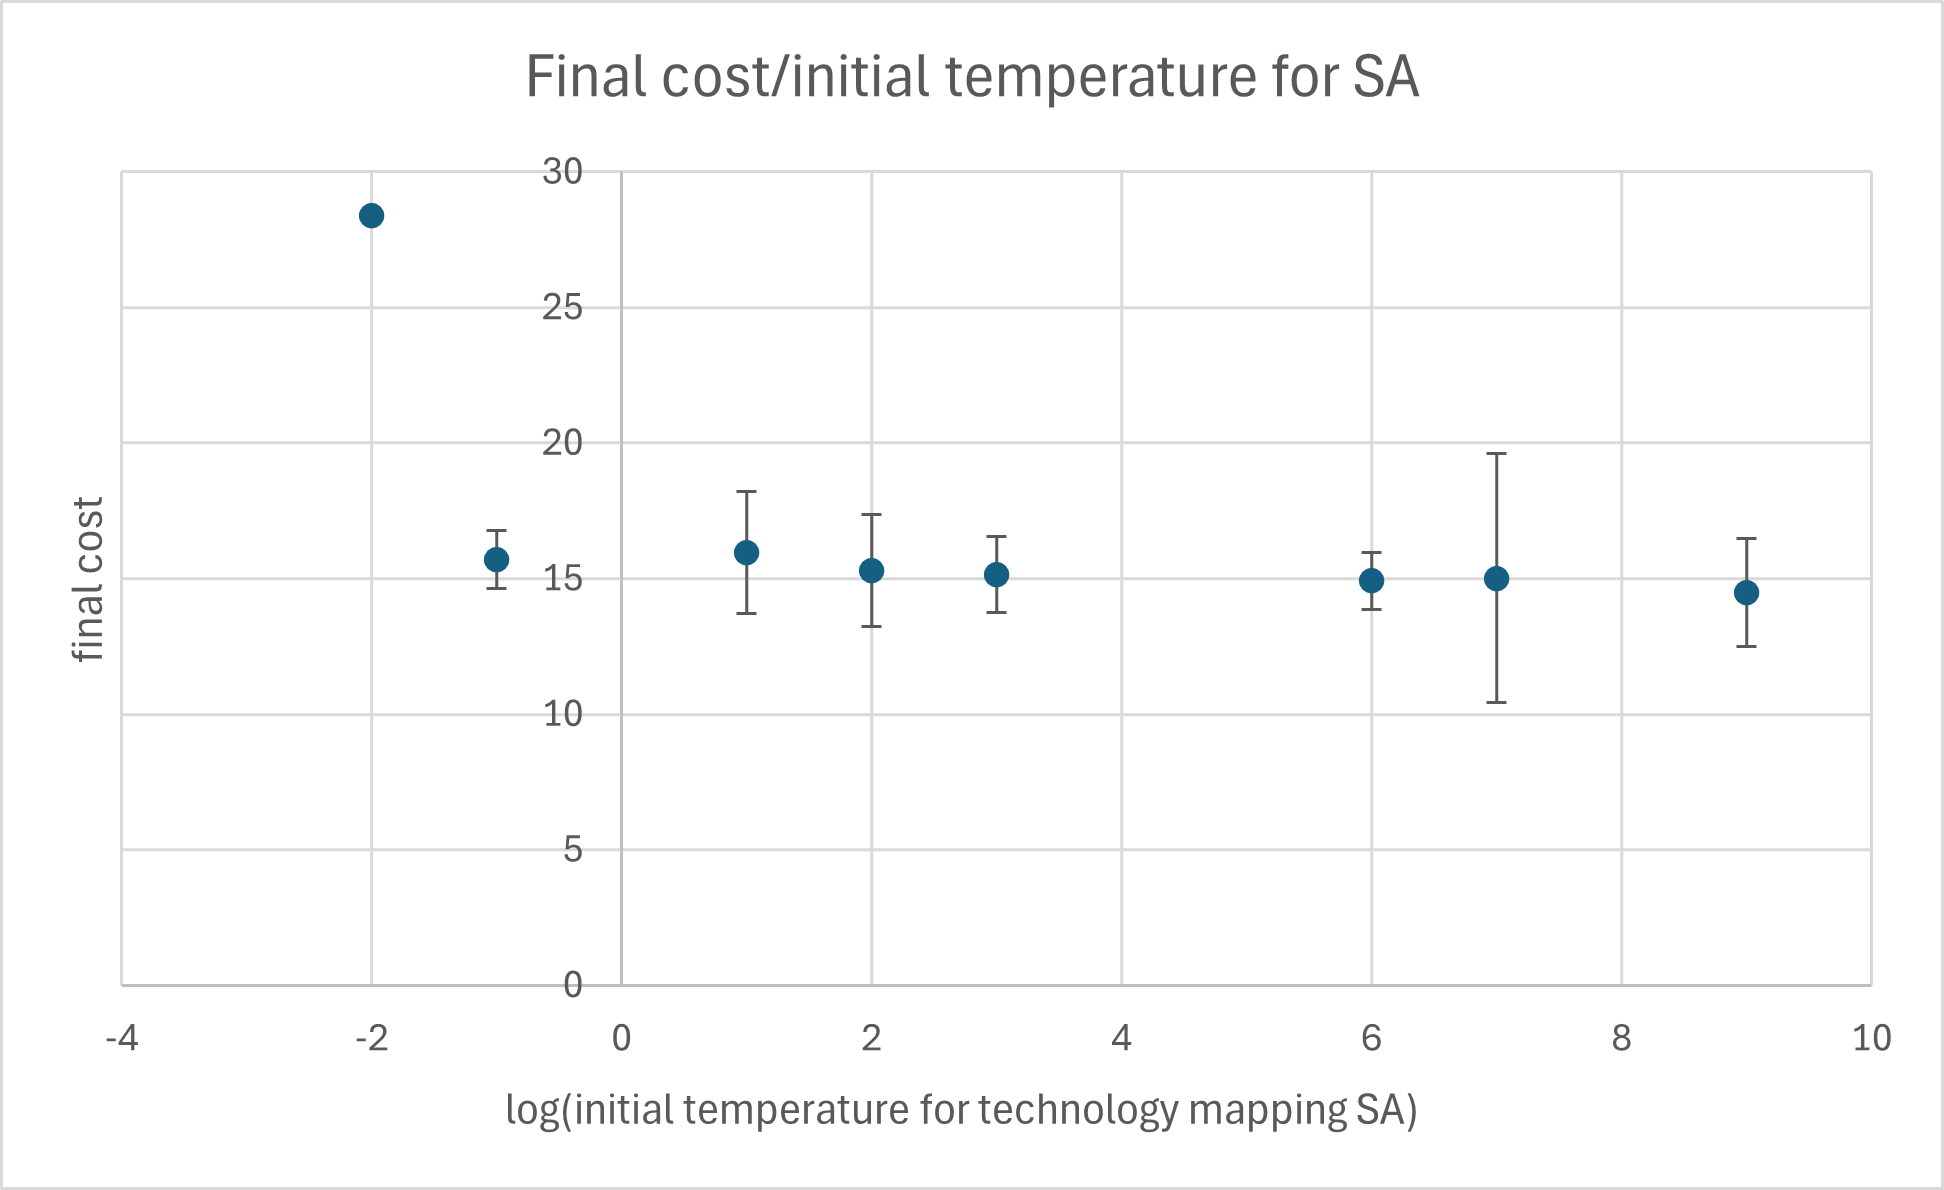
\includegraphics[width=0.9\linewidth]{cost.png}
    \caption{Result with different initial temperature for SA}
    \label{fig:enter-label}
\end{figure}

\section{Future works}
Future work may involve incorporating reinforcement learning techniques into the model, as they have demonstrated significant potential. Additionally, our current model does not consider the parameters of all gates, as we employed a greedy method (Find Suitable Gates) to determine which gates to use. By integrating these two components, we may achieve better results.

\section{Job division}
\begin{itemize}
    \item B11901015 Ssuwei Huang: meta-model structure, code reconstruction, ABC-related programming, resolution of git-related issues, report.
    \item B11901020 Boyuan Cheng: data extraction from Verilog file, gate selection, SA analysis based on temperature, performance recording, report.
    \item B11901027 Renxuan Wang: ICCAD registration, programming for LSA and TSA, adjustment of simulated annealing parameters, generation of Verilog-format results, report.
\end{itemize}

\begin{thebibliography}{00}
\bibitem{b1} ABC: System for Sequential Logic Synthesis and Formal Verification. https://github.com/berkeley-abc/abc
\bibitem{b1} ICCAD Cad Contest: Reinforcement Logic Optimization for a General Cost Function. https://drive.google.com/file/d/1AfxpS7q7OEg5QP06wgk1rrVqZroT7Ypi/view
\end{thebibliography}
\end{document}
